\documentclass[12pt]{article}

\usepackage{amsmath}
\usepackage[margin=1in]{geometry}
\usepackage{hyperref}
\usepackage{graphicx}
\usepackage[backend=biber]{biblatex}
\addbibresource{paper.bib}
\graphicspath{{./images/}}
\linespread{2}

\usepackage{pythontex}
\newcommand{\ohsheader}[3]{ #1 \par
    #2 \par %class
    \today \par
    #3 %assignment
}

\title{An Analysis of Visual Subitization Across Different Modes of Peripheral
Vision}

\author{Juni Kim \\
Stanford Online High School}

\date{\today}

\begin{document} 

\maketitle

Subitization is the almost instantaneous ability of humans to visually deduce
the quantity of a group or category of objects given that the number is small
enough. For numbers beyond four, humans will instinctually use either a
system of approximation that is less accurate or an effortful, time-consuming
counting strategy. When one uses this process of subitizing, they are able to
recognize the numerosity of objects without counting, as if it were an
alternate form of perception.  In this study, I examined the human’s
fundamental skills in “number sense” by testing the effect of visual perception
on one’s ability to precisely subitize a small group of objects. 

Peripheral vision is the ability of humans to see objects that are outside the
focus of the eye. Although central vision within the focus requires most of our
mental resources, such as memory and attention, and allows us to see things
with sharp detail, peripheral vision enables us to view objects around the
entire visual field. Peripheral vision is also a vital component of detecting
motions and changes and supports functions of the central vision. Vision
scientists have shown that peripheral vision has relatively poor resolution and
acuity compared to central vision. Testing one’s ability to subitize the number
of objects presented to the peripheral vision compared to central vision will
thus unveil whether or not visual resolution has a significant effect on
subitization ability.

In my final project for OMSB9, I collected and analyzed data to evaluate the
ability of people to accurately subitize the number of objects in a drawing
along different angles of vision and the time in which an image was presented.
I intend to find the accuracy of subitizing across different modes of
peripheral vision and effects of the presentation duration on participants'
performance.

\section{Methodology}

\subsection{Samples}
A sample of 5 people was used in this experiment (due to the lack of reachable
people as a result of COVID-19). I conducted tests on 4 different durations (250ms,
500ms, 750ms, and 1000ms) and 3 different angles relative to straight ahead
($0^{\circ}$ for central presentation and $30^{\circ}$ and $60^{\circ}$ for near and far-peripheral presentation, respectively), leading to a net 12 different
variations on the test to perform. Each of these variations was done five times
per participant.

\subsection{Scripts}

In order to make the testing procedure more efficient, I wrote a set of PHP
scripts that could be run in a localhost setting and allow me to both run and record the
tests. The source code can be found in
\href{https://github.com/junikimm717/OMSB9-Final-Project}{this link}.

\subsubsection{Testing Page}
The testing page is located in the /testing.php file.

Within the testing page, one may modify the GET parameters (which include the
participant name, angle being tested, and the time being tested) to
conduct different tests. When one clicks the ``conduct test" button, a randomly
selected picture (consisting of a certain number of clearly visible dots) will
appear for a duration of time equal to the one that was put in the GET
parameters. The participant was asked how many dots they believed (to their
best guesses) were in the picture that was flashed, and their response
was recorded. Once the test was complete, the ``submit" button was clicked.

\subsubsection{Handler Page}
The handler is located in the /handler.php file.

The handler page records all of the data gained from the test through a POST
request (so that a particularly adept participant cannot simply scan the GET
parameters and evaluate their previous answers) and appends this data
into a file called data.txt (note that the file never gets overwritten).

The handler page also contains a pre-filled HTML form which I could
modify if I wanted to change the settings for the next test.

\subsection{Physical Setup}
A sheet of 11x17 paper was used to make demarcations of 0, 30, and 60 degree
deviations from the center of the screen in order to consistently align the
monitor correctly. At the 0 degree line, an object would be placed (preferably
one that is relatively thin) for the participant to focus their fovea
on while the test is taking place.  The computer was then placed on one of the
lines (for testing a particular angle), and the test was initiated.


\begin{figure}
\centering
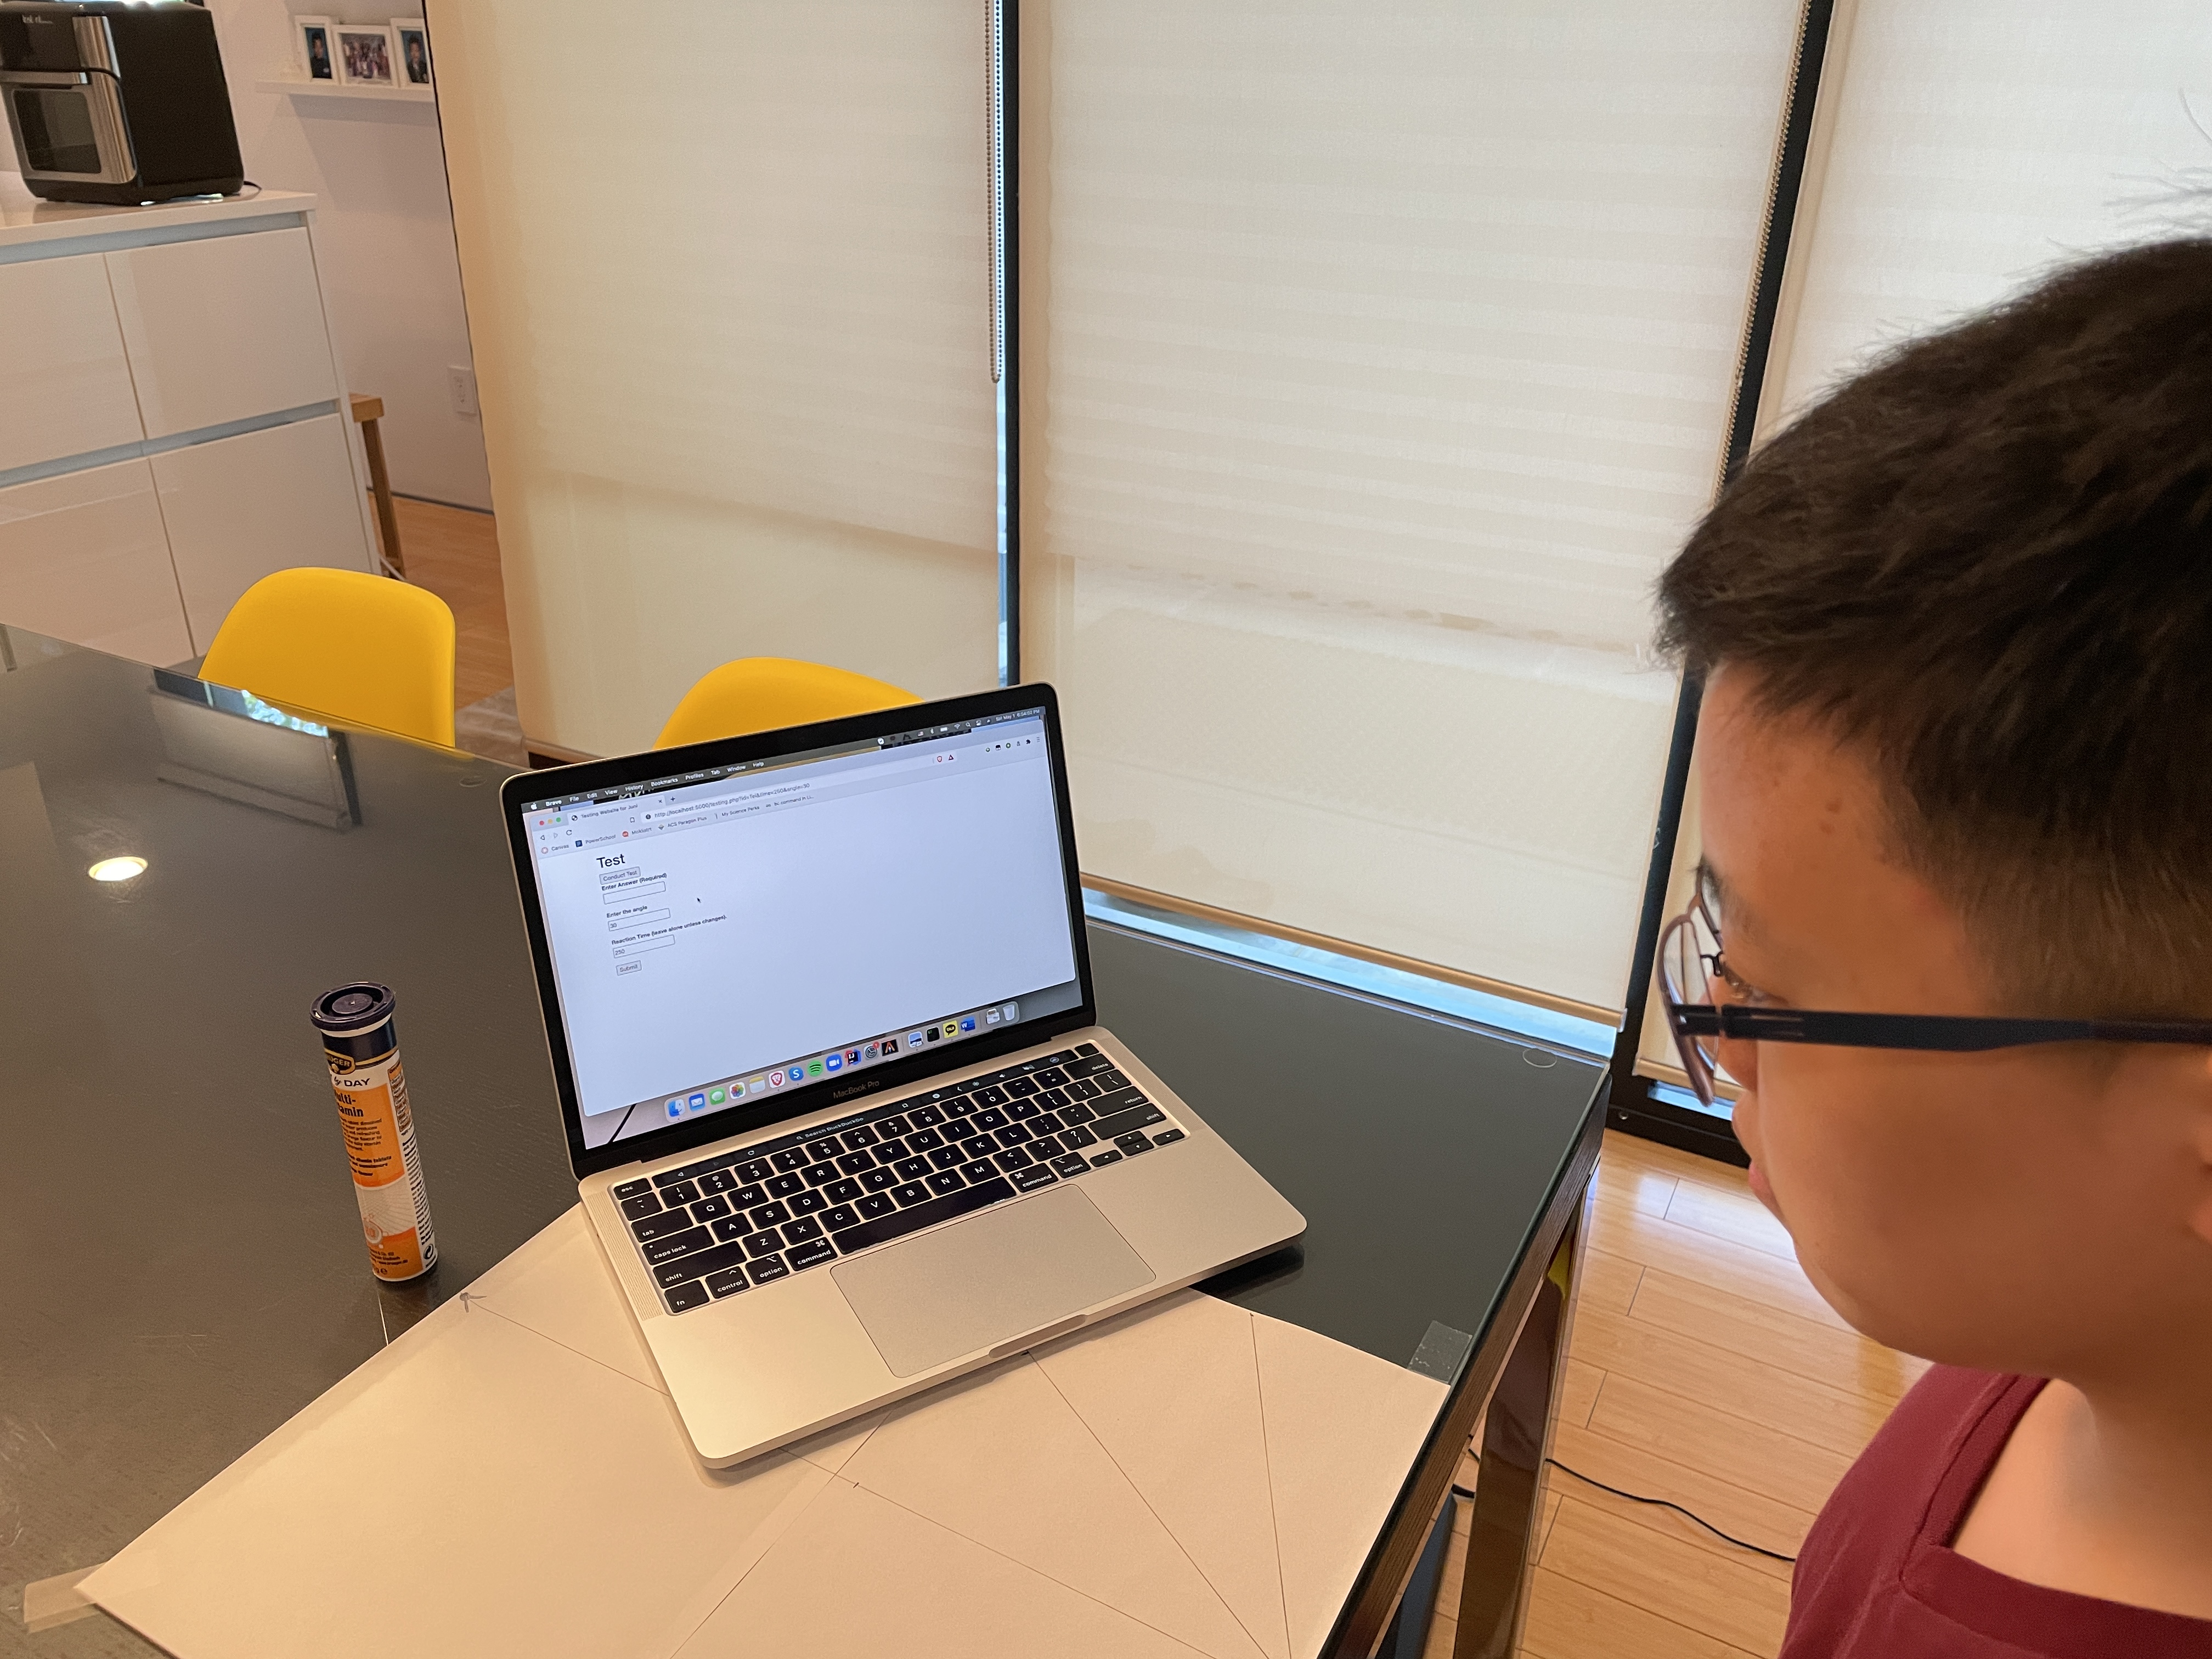
\includegraphics[scale=0.3]{diagram.JPG}
\caption{How the experiment should appear}
\end{figure}

\section{Data}
The raw (unprocessed) data can be found at \\
\url{https://github.com/junikimm717/OMSB9-Final-Project/tree/main/data/data.txt}
The data points seen below were all generated with matplotlib.

\begin{figure} [p]
\centering
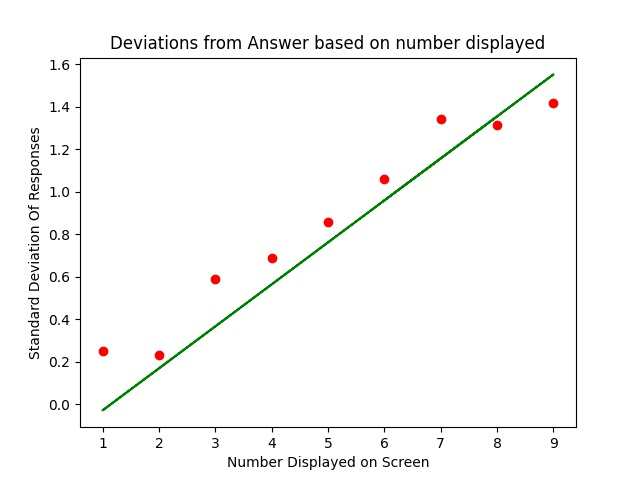
\includegraphics[scale=0.4]{regression.jpg}
\caption{Standard Deviation of Responses}
\end{figure}

\begin{figure} [p]
\centering
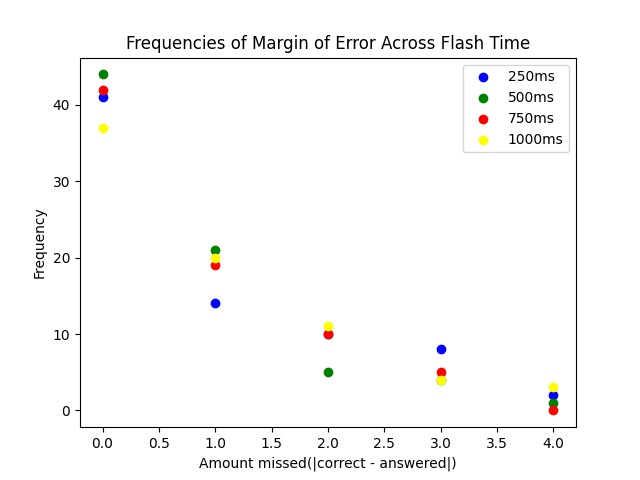
\includegraphics[scale=0.4]{reaction.jpg}
\caption{Accuracy across different flash times}
\end{figure}

\begin{figure} [p]
\centering
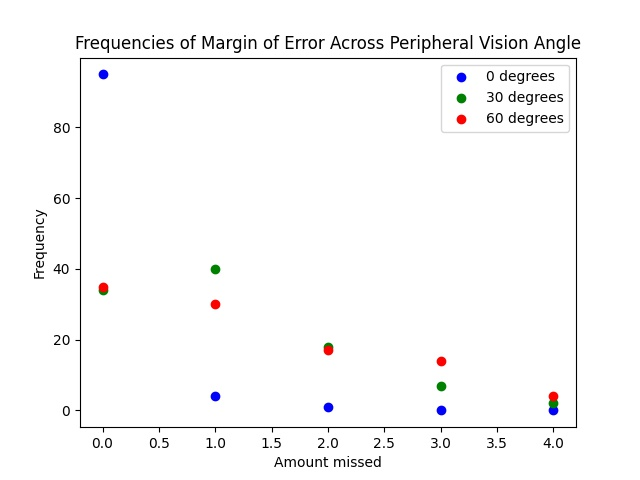
\includegraphics[scale=0.4]{angle.jpg}
\caption{Accuracy across different angles}
\end{figure}

\newpage
\section{Analysis}

Based on the raw data, I have been able to perform some analyses to address my
research question on the effects of the visual angle and stimulus duration on
participants’ subitizing performance. 

\subsection{Deviations from answer}

For assessing the standard deviations of participants' responses per answer
(the actual number of dots displayed), a linear regression was plausible
because there was minimal likelihood that the standard deviation of responses
would have a non-consistent distribution per response.

In addition, previously cognitive psychologists have found that estimation
variability grows proportionally to the number of items displayed (\cite{prop})

A product moment correlation test assessing the correlation between the correct
answer and the standard deviation of responses exhibits a p-value of $2.1 \cdot
10^{-5}$ seems to indicate that there exists a statistically highly significant
positive correlation.

\subsection{Accuracy Based on Time Flashed (Figure 3)}

For assessing this correlation, I used a Spearman rank correlation coefficient
(a non-parametric test) in order to assess if there was a significant monotonic
correlation between precision of the participant and the average flash time.

The Spearman rank test statistic was equal to 0.027 and the p-value was 0.638,
which indicates that, with the data collected, there is no statistically
significant monotonic correlation between the time given for the
participant to look at the image and their precision.

This result indicates that participants’ subitizing accuracy was not affected
by the different presentation durations in this experiment. Thus, the shortest
duration (250 msec) appeared to be sufficient for subitization to be as
accurate as in the longest duration (1000 msec).

\subsection{Accuracy based on Angle Viewed (Figure 4)}

In order to assess whether or not participants were significantly accurate on
at least one of the three angles at which they were tested, I conducted
a one-way ANOVA test (as the data is both parametric and has multiple samples).

The results show that $F=47.5$ and $p = 1.23 \cdot 10^{-18}$, which indicates
that there is a statistically highly significant difference between the results
across different angles.

As an additional note, because the errors for 0 degree (with a peak at around
$0.0$ in Figure 4) was smaller than those for the 30 and 60 degrees,
this result suggests that the participants’ subitization performance
impaired with greater visual angle of the presentation.

\subsection{Near Peripheral Vision vs Far Peripheral Vision?}

In order to test whether or not near peripheral vision yielded a statistically
significantly better precision, I used a two-sample t-test.

The results indicated that $T = -1.707$ and $p = 0.121$, which indicates that
there was no statistically significant difference between precision when
participants viewed the pictures from $30^{\circ}$ versus $60^{\circ}$.

\section{Conclusions}
Based on the data collected and statistically analyzed in this study, I have
been able to prove that the mean precision is different among tests from
different angles of vision (Section 3.3).  However, I have been unable to prove
such a difference exists between near and far peripheral vision (Section 3.4).
As a benchmark, we have also shown a statistically significant linear
correlation between the amount of error within the participants' tests and the
number that was displayed in front of them, which indicates (as others have
previously shown), that the ability of subitization decreases as one
sees more objects that they must perceive.

As I had constraints of time and accuracy as a result of being within the
COVID-19 pandemic, I was unable to get a larger set of peripheral vision angles
to check, which might have allowed me to do a correlation analysis and thus
gain better insights. Other studies might also be able to obtain more
volunteers than I have been able to.

There were also constraints from the programs that I used to run the tests. As
I used browser javascript to flash the images, there were rendering issues
within the browser once I set the flash time to below 150ms. It is possible
that using a faster GUI program written in a faster environment would have
allowed me to more closely examine the correlations between flash time and
subitization ability.

\printbibliography

\end{document}
